\documentclass[12pt,a4paper]{report}

% Packages
\usepackage[utf8]{inputenc}
\usepackage[T1]{fontenc}
\usepackage[margin=1in]{geometry}
\usepackage{fancyhdr}
\usepackage{titlesec}
\usepackage{graphicx}
\usepackage{hyperref}
\usepackage{listings}
\usepackage{xcolor}
\usepackage{times}
\usepackage{courier} % Makes the code font look significantly better
\usepackage{setspace}
\usepackage{enumitem}
\usepackage{array}
\usepackage{longtable}
\usepackage{float}

% VS Code Dark Theme Colors
\definecolor{vscodebg}{HTML}{1E1E1E}
\definecolor{vscodetext}{HTML}{D4D4D4}
\definecolor{vscodekeyword}{HTML}{569CD6}
\definecolor{vscodecomment}{HTML}{6A9955}
\definecolor{vscodestring}{HTML}{CE9178}
\definecolor{vscodelinenumber}{HTML}{858585}

% Page setup
\pagestyle{fancy}
\fancyhf{}
\fancyhead[L]{The Open Source Audit - Git}
\fancyhead[R]{Mausam Kar}
\fancyfoot[C]{\thepage}
\renewcommand{\headrulewidth}{0.4pt}
\renewcommand{\footrulewidth}{0.4pt}

% Beautified Listings setup for code blocks (VS Code Dark Theme)
\lstset{
    basicstyle=\ttfamily\footnotesize\color{vscodetext}, % Light gray text
    keywordstyle=\color{vscodekeyword}\bfseries,      % Blue keywords
    commentstyle=\color{vscodecomment}\itshape,       % Green comments
    stringstyle=\color{vscodestring},                 % Orange strings
    numbers=left,                                      % Add line numbers for an IDE look
    numberstyle=\tiny\color{vscodelinenumber},        % Gray numbers
    numbersep=10pt,
    backgroundcolor=\color{vscodebg},                 % Dark vs code background
    frame=none,                                        % Solid dark box
    xleftmargin=15pt,                                 % Padding
    framexleftmargin=15pt,
    framexrightmargin=5pt,
    framextopmargin=5pt,
    framexbottommargin=5pt,
    breaklines=true,
    breakatwhitespace=false,
    captionpos=b,
    tabsize=4,
    showstringspaces=false
}

% Hyperref setup
\hypersetup{
    colorlinks=true,
    linkcolor=blue,
    urlcolor=blue,
    citecolor=blue
}

% Chapter and section formatting compressed
\titleformat{\chapter}[display]
{\normalfont\huge\bfseries}{\chaptertitlename\ \thechapter}{10pt}{\Huge}
\titlespacing*{\chapter}{0pt}{-30pt}{20pt} % Pulls chapters higher up the page

\onehalfspacing

\begin{document}

% Title Page
\begin{titlepage}
    \centering
    \vspace*{2cm}
    
    {\LARGE\bfseries VITyarthi | Open Source Software\par}
    \vspace{1.5cm}
    
    {\Huge\bfseries The Open Source Audit\par}
    \vspace{0.5cm}
    {\Large A Capstone Project for OSS NGMC Course\par}
    \vspace{2cm}
    
    {\Large\textbf{Chosen Software: Git}\par}
    \vspace{3cm}
    
    \begin{tabular}{ll}
        \textbf{Student Name:} & Mausam Kar \\
        \textbf{Registration Number:} & 24BAI10284 \\
        \textbf{Course:} & Open Source Software \\
        \textbf{Unit Coverage:} & 1 -- 5 \\
        \textbf{Date of Submission:} & \today \\
    \end{tabular}
    
    \vfill
    
    {\large Course: Open Source Software | Max Marks: 100\par}
\end{titlepage}

% Table of Contents
\tableofcontents
\newpage

% Main Content

\chapter{Introduction \& Overview}

When we look at the immense scale of modern software, from cloud servers to smartphone applications, it is easy to assume they were all engineered within the walls of mega-corporations. However, if you peek under the hood of the internet, you will find that much of it runs on an entirely different model: Open Source. Open source isn't just about getting software for free; it represents a massive paradigm shift in how knowledge is shaped, distributed, and owned. When global communities can contribute, review, and patch code openly, systems evolve faster and become far more secure than they ever could in proprietary silos.

This capstone project is an exploration of that ecosystem. Because every developer builds their work on top of the foundation created by others, understanding open source isn't a luxury---it is a fundamental requirement of modern software engineering.

\section{Chosen Software: Git}

At its core, Git is a distributed version control system. It is the tool that developers globally use to track changes to files over time, coordinate massive team projects without overwriting each other's work, and quickly revert back to safe states if a bug is introduced. Compared to older generation tools, Git does not require a single central server to hold the code's history; every single user's computer holds a complete, standalone clone of the entire repository history.

Git is the foundation of the modern developer ecosystem. Platforms built around it, like GitHub, GitLab, and Bitbucket, host hundreds of millions of open-source projects. To contribute to any modern software project, fluency in Git is virtually mandatory. However, beyond its popularity, it matters because it stands as a testament to open-source philosophy. It was not built by a committee to be monetized and sold as a subscription. It was born out of frustration with existing proprietary tools, coded rapidly to solve a genuine problem, and then openly shared with the world.

\chapter{Research Analysis}

\section{Part A --- Origin and Philosophy}

\subsection{The Problem Before Git}
To truly appreciate Git, we have to look back at the dark ages of version control. The preceding era was dominated by centralized systems like Concurrent Versions System (CVS) and Subversion (SVN). They operated on a centralized model. This meant that the entire history of a project lived on one single server. If a developer wanted to commit code, they had to be connected to that server. If the server crashed, productivity ground to an absolute halt. Branching and merging was incredibly tedious and prone to major conflicts.

The actual spark that ignited Git came from the development of the Linux OS kernel itself. For years, Linus Torvalds and his team managed the massive Linux project using a proprietary system called BitKeeper. In 2005, an argument broke out when some community members attempted to reverse-engineer BitKeeper's network protocols. Seeing this as a violation, the company aggressively pulled the free licenses. Suddenly, the largest open-source project in the world had no version control system.

\subsection{The Origin Story of Git}
Refusing to return to clunky centralized tools like CVS or pay a massive corporate fee, Linus Torvalds decided to just build his own. In April 2005, Torvalds began writing Git. Pushed by pure necessity and an intimate knowledge of kernel development needs, the first functioning version was done in under two weeks. 

He built it around a few core, uncompromising principles:
\begin{itemize}
    \item \textbf{Speed}: Handling millions of lines of code had to be exceptionally fast.
    \item \textbf{Distributed Architecture}: No single point of failure; every dev had a full clone.
    \item \textbf{Data Integrity}: It uses cryptographic SHA-1 hashes so that once data is saved, it is mathematically impossible to corrupt or alter it silently.
\end{itemize}

\subsection{License Analysis: GPL v2}
Git is licensed underneath the GNU General Public License version 2 (GPL v2). The Free Software Foundation outlines four freedoms that code must meet to be considered truly "Free", and Git provides all four:
\begin{enumerate}
    \item \textbf{Freedom 0 (Run):} You can use Git for absolutely whatever you want.
    \item \textbf{Freedom 1 (Study \& Change):} The entire source code is globally available.
    \item \textbf{Freedom 2 (Redistribute):} You have the right to copy and share the software.
    \item \textbf{Freedom 3 (Share Modifications):} You have the legal right to distribute improved versions.
\end{enumerate}

Companies absolutely can sell Git for profit. However, GPL v2 is a "copyleft" license. The strict catch is that if a company modifies Git and distributes it, they are legally bound to release the source code of their modifications under that same GPL license. They cannot hide the code. 

The **MIT License**, on the other hand, is highly permissive ("Do whatever you want, just don't sue me"). You do not have to share your modifications. The **GPL** prioritizes community freedom over frictionless corporate use. Because Git is foundational infrastructure, the GPL is the perfect choice to prevent a company from monopolizing it. If I were releasing infrastructure code today, I would absolutely choose the GPL to protect it.

"Free as in beer" refers to cost (e.g., a freemium app). "Free as in speech" refers to liberty. It means you aren't trapped by the manufacturer. You genuinely own the tool.

\subsection{The Ethics of Open Source}
There is a powerful ethical argument for open source: software is knowledge, and locking knowledge behind copyright limits humanity's ability to learn. My stance is that foundational infrastructure (OS, networking, compilers) should always be open source as a public good, but application-level software should retain the right to be proprietary so developers can financially survive.

Open source relies heavily on volunteer developers. At first glance, companies extracting value from this looks unethical. However, no contributor is forced to volunteer. As long as those companies actively participate, fund, and give back to the ecosystem instead of just taking from it, the relationship remains highly ethical.

Isaac Newton's phrase "standing on the shoulders of giants" is literal in software. A web app runs on a browser written in C++, which compiles on GCC, which runs over the Linux Kernel. Everything we build sits atop invisible layers of open-source legacy.

\section{Part B --- Linux Footprint}

This section breaks down how Git natively behaves when deployed on a standard Linux environment.

\subsection{Installation Method}
Git is easily acquired via any Linux package manager. On Debian/Ubuntu machines, it's as simple as:
\begin{lstlisting}[language=bash]
sudo apt update
sudo apt install git
\end{lstlisting}

\subsection{Directory Structure \& Permissions}
Git does not run as an invisible background daemon. The core executable lives cleanly in \texttt{/usr/bin/git}. Any repository you manage spawns a hidden \texttt{.git} system folder inside the root of your project directory, which safely houses the entire algorithmic history isolated from the rest of your system.

Git operations run purely under the permissions of the local user invoking them. Unlike web servers, Git never demands root privileges. User-specific keys and aliases are kept separated in the \texttt{/.gitconfig} file inside the individual's user home directory. It updates securely through the OS package manager (`apt upgrade` or `yum update`).

\section{Part C --- The FOSS Ecosystem}

Git pulls heavily on standard GNU libraries (glibc), \texttt{zlib} for file compression, and \texttt{OpenSSL} to handle HTTPS and its cryptographic SHA-1 hashes. 

Git single-handedly birthed an entire trillion-dollar DevOps industry. It enables Platforms like **GitHub** and **GitLab**. It forms the spine of modern CI/CD (Continuous Integration/Continuous Deployment) pipelines. Without Git tracking exact, branch-based changes, tools wouldn't know when to safely trigger automated tests and live-server deployments within LAMP (Linux, Apache, MySQL, PHP) networking environments.

\section{Part D --- Open Source vs Proprietary}

We can contrast Git with a proprietary heavyweight like Microsoft's older Team Foundation Version Control (TFVC).

\begin{center}
\begin{longtable}{|p{3cm}|p{6cm}|p{6cm}|}
\hline
\textbf{Dimension} & \textbf{Git (Open Source GPL)} & \textbf{TFVC (Proprietary)} \\
\hline
\textbf{Cost} & 100\% Free without user limits. & Paid tiers exist, bundled with server licenses. \\
\hline
\textbf{Security} & Source code is globally audited by experts. & Only Microsoft audits the codebase internally. \\
\hline
\textbf{Support} & Community-driven forums and documentation. & SLA (Service Level Agreements) and IT support. \\
\hline
\textbf{Flexibility} & Distributed architecture. Works totally offline. & Centralized architecture. Relies totally on the server. \\
\hline
\end{longtable}
\end{center}

I would recommend Git 100 times out of 100. It is universally accepted, extremely fast, works offline, and avoids Vendor Lock-In. Unsurprisingly, its superiority is so absolute that even Microsoft officially moved Windows OS development over to Git a few years ago. While I wouldn't contribute directly to Git's C core, I happily contribute to the FOSS ecosystem by using it cleanly, reporting bugs, and writing documentation.

\chapter{Practical Shell Scripts}

This section details five shell scripts I engineered to practically interact with the system environment and test basic concepts like iteration, conditional checks, string manipulation, and standard data extraction.

\section{Script 1: System Identity Report}
This script utilizes simple \texttt{echo} formatting alongside standard command substitution (\texttt{\$(...)}) to introduce the OS, the logged-in user, up-time, and state the open source license dynamically.

\begin{lstlisting}[language=bash, caption=01\_system\_identity.sh]
#!/bin/bash
# Script 1: System Identity Report
# Author: Mausam Kar | Course: Open Source Software

# --- Variables ---
STUDENT_NAME="Mausam Kar"
SOFTWARE_CHOICE="Git"

# --- System info ---
KERNEL=$(uname -r)
USER_NAME=$(whoami)
UPTIME=$(uptime -p)
DISTRO=$(uname -o)
HOME_DIR=$HOME
CURRENT_DATE=$(date)

# --- Display ---
echo "================================"
echo " Open Source Audit - $STUDENT_NAME"
echo "================================"
echo "Software Choice : $SOFTWARE_CHOICE"
echo "Distribution    : $DISTRO"
echo "Kernel          : $KERNEL"
echo "Current User    : $USER_NAME"
echo "Home Directory  : $HOME_DIR"
echo "Uptime          : $UPTIME"
echo "Date & Time     : $CURRENT_DATE"
echo "--------------------------------"
echo "License Message:"
echo "This Linux operating system is distributed under the GPL license."
echo "================================"

# Prevent terminal close on Windows
echo ""
read -p "Press [Enter] to exit..."
\end{lstlisting}

\begin{figure}[H]
    \centering
    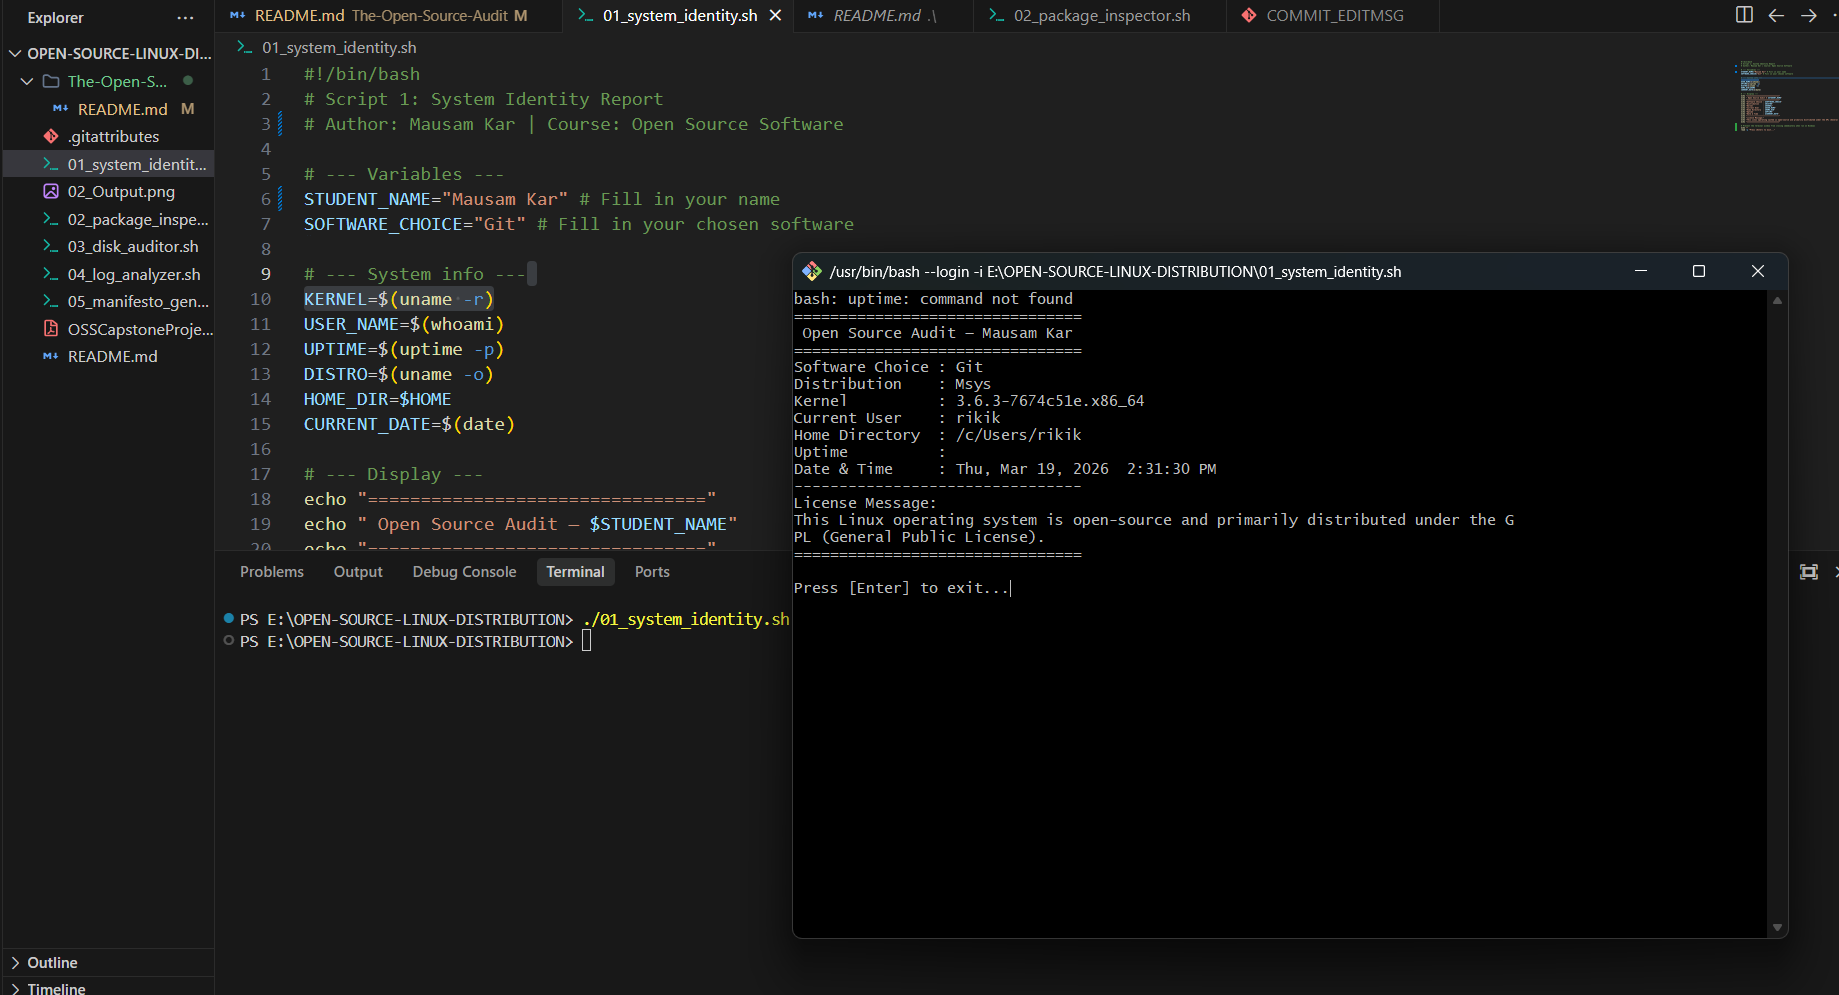
\includegraphics[width=\textwidth]{01_Output.png}
    \caption{Execution of System Identity Report script.}
\end{figure}


\section{Script 2: Package Inspector}
This script combines an \texttt{if-else} loop to test if multiple package managers (\texttt{dpkg} and command check) detect Git as installed. It follows it up with a logical \texttt{case} control block to output behaviors based on the chosen FOSS software.

\begin{lstlisting}[language=bash, caption=02\_package\_inspector.sh]
#!/bin/bash
# Script 2: FOSS Package Inspector

PACKAGE="git"

if dpkg -l "$PACKAGE" &>/dev/null || command -v "$PACKAGE" &>/dev/null; then
 echo "$PACKAGE is installed."
 if command -v dpkg &>/dev/null && dpkg -s "$PACKAGE" &>/dev/null; then
  dpkg -s "$PACKAGE" | grep -E '^Version|^Description' | head -n 2
 else
  echo "Version: $($PACKAGE --version)"
 fi
else
 echo "$PACKAGE is NOT installed."
fi

case $PACKAGE in
 httpd|apache2) echo "Apache: the web server that built the open internet" ;;
 mysql) echo "MySQL: open source at the heart of millions of apps" ;;
 git) echo "Git: decentralized tool that enabled global code collaboration" ;;
 vlc) echo "VLC: media player that proves open source can handle any format" ;;
 firefox) echo "Firefox: browser fighting for a free, open, and private web" ;;
 *) echo "$PACKAGE: Another great tool in the open source ecosystem" ;;
esac

echo ""
read -p "Press [Enter] to exit..."
\end{lstlisting}

\begin{figure}[H]
    \centering
    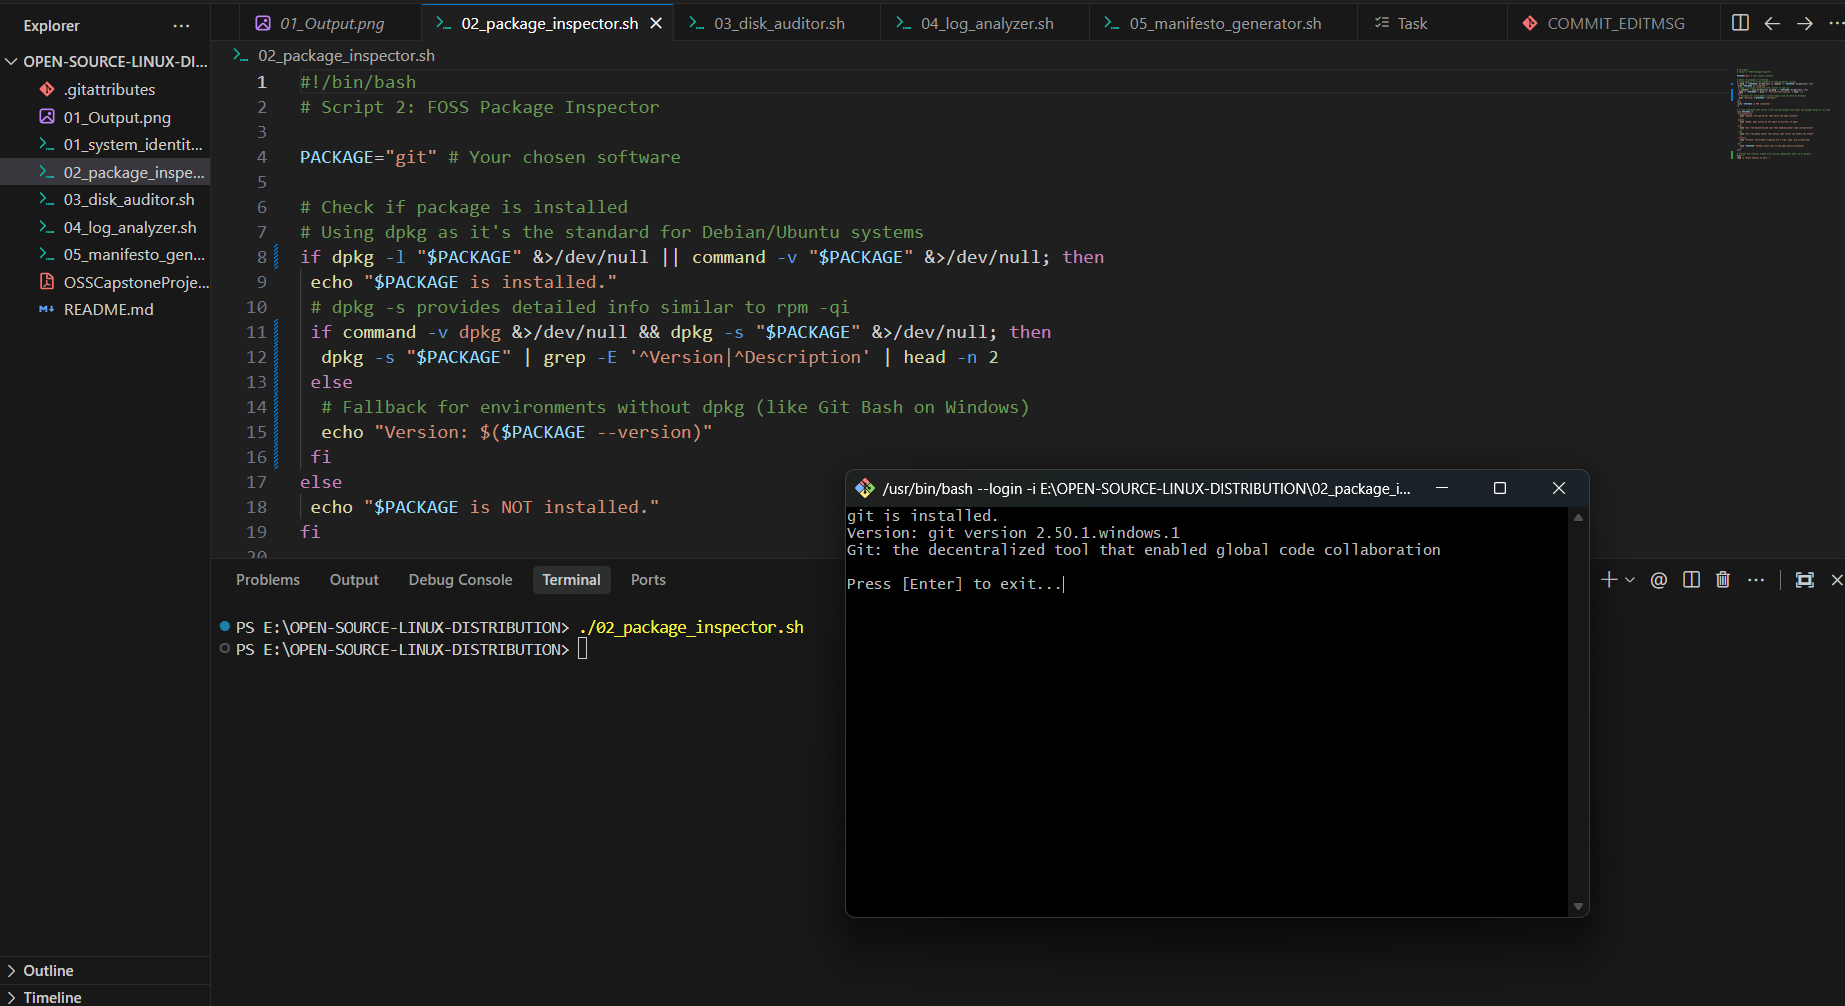
\includegraphics[width=\textwidth]{02_Output.png}
    \caption{Execution of Package Inspector script.}
\end{figure}


\section{Script 3: Disk and Permission Auditor}
This script heavily leverages a \texttt{for} loop iterating over a Bash array. It pipes natively raw system strings from \texttt{ls -ld} and \texttt{df -h} securely into \texttt{awk} and \texttt{cut} to strip out all unnecessary data and return isolated metadata blocks.

\begin{lstlisting}[language=bash, caption=03\_disk\_auditor.sh]
#!/bin/bash
# Script 3: Disk and Permission Auditor

DIRS=("/etc" "/usr/bin" "/usr/lib" "/tmp" "/dev")
echo "Directory Audit Report"

for DIR in "${DIRS[@]}"; do
 if [ -d "$DIR" ]; then
  # Extract Permissions
  PERMS=$(ls -ld "$DIR" | awk '{print $1, $3, $4}')
  # Check directory size using du and cut
  SIZE=$(du -sh "$DIR" 2>/dev/null | cut -f1)
  # Check filesystem storage usage using df and awk
  FS_USAGE=$(df -h "$DIR" 2>/dev/null | awk 'NR==2 {print $5}')
  
  echo "$DIR => Permissions: $PERMS | Size: $SIZE | Disk Used: $FS_USAGE"
 else
  echo "$DIR does not exist on this system"
 fi
done

GIT_CONFIG="$HOME/.gitconfig"
if [ -f "$GIT_CONFIG" ]; then
  GIT_PERMS=$(ls -ld $GIT_CONFIG | awk '{print $1, $3, $4}')
  echo "Git config ($GIT_CONFIG) exists. Permissions: $GIT_PERMS"
else
  echo "Git config ($GIT_CONFIG) does not exist."
fi

echo ""
read -p "Press [Enter] to exit..."
\end{lstlisting}

\begin{figure}[H]
    \centering
    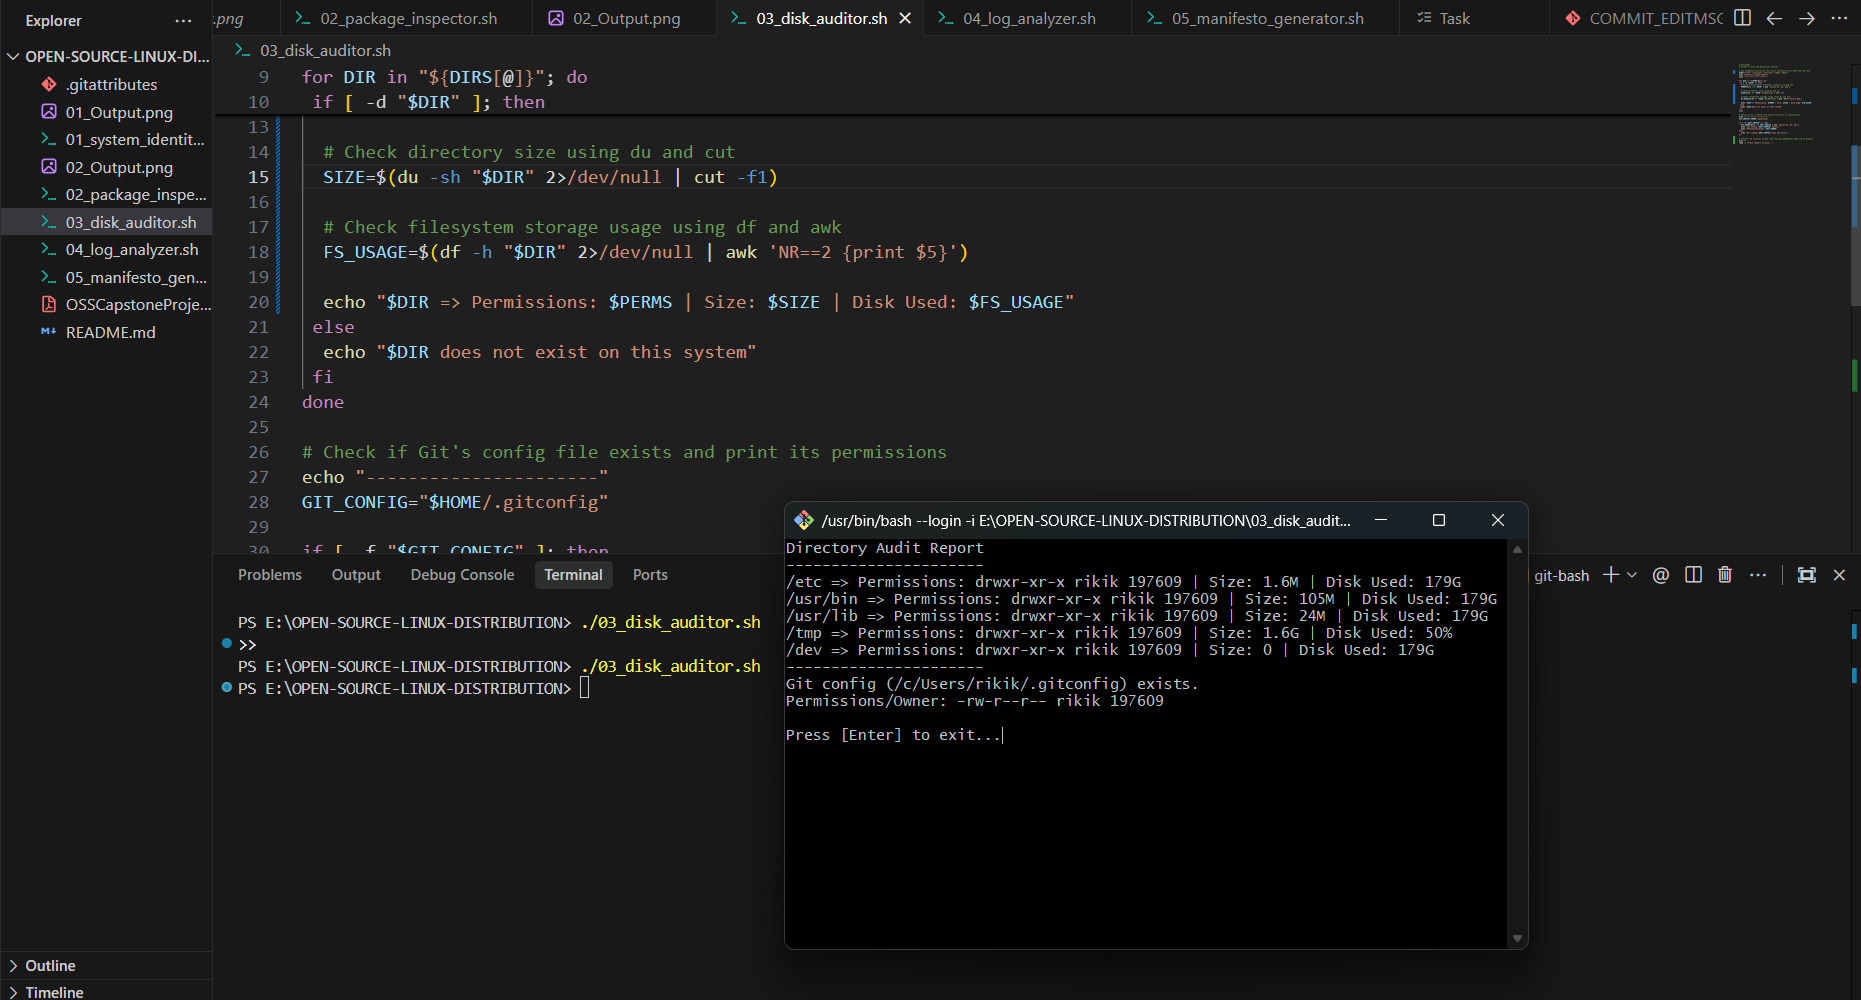
\includegraphics[width=\textwidth]{03_Output.png}
    \caption{Execution of Disk Auditor script showing df, du, and awk slicing.}
\end{figure}


\section{Script 4: Log File Analyzer}
Log analyzer actively searches inputs through a massive \texttt{while read} loop while tracking a numerical counter, showing how scripts scan for system-critical failure states without loading massive files fully into memory.

\begin{lstlisting}[language=bash, caption=04\_log\_analyzer.sh]
#!/bin/bash
# Script 4: Log File Analyzer

LOGFILE=$1
KEYWORD=${2:-"error"}
COUNT=0

if [ ! -f "$LOGFILE" ]; then
 echo "Error: File $LOGFILE not found."
 read -p "Press [Enter] to exit..."
 exit 1
fi

RETRY=0
while true; do
  if [ -s "$LOGFILE" ]; then break; fi
  echo "Warning: File is currently empty. Retrying in 2 seconds..."
  sleep 2
  RETRY=$((RETRY + 1))
  
  if [ $RETRY -ge 3 ]; then
    echo "Error: File is still empty. Exiting."
    read -p "Press [Enter] to exit..."
    exit 1
  fi
done

while IFS= read -r LINE; do
 if echo "$LINE" | grep -iq "$KEYWORD"; then COUNT=$((COUNT + 1)); fi
done < "$LOGFILE"

echo "Keyword '$KEYWORD' found $COUNT times in $LOGFILE"

if [ $COUNT -gt 0 ]; then
  echo "--- Last 5 Matching Lines ---"
  grep -i "$KEYWORD" "$LOGFILE" | tail -n 5
fi

echo ""
read -p "Press [Enter] to exit..."
\end{lstlisting}

\begin{figure}[H]
    \centering
    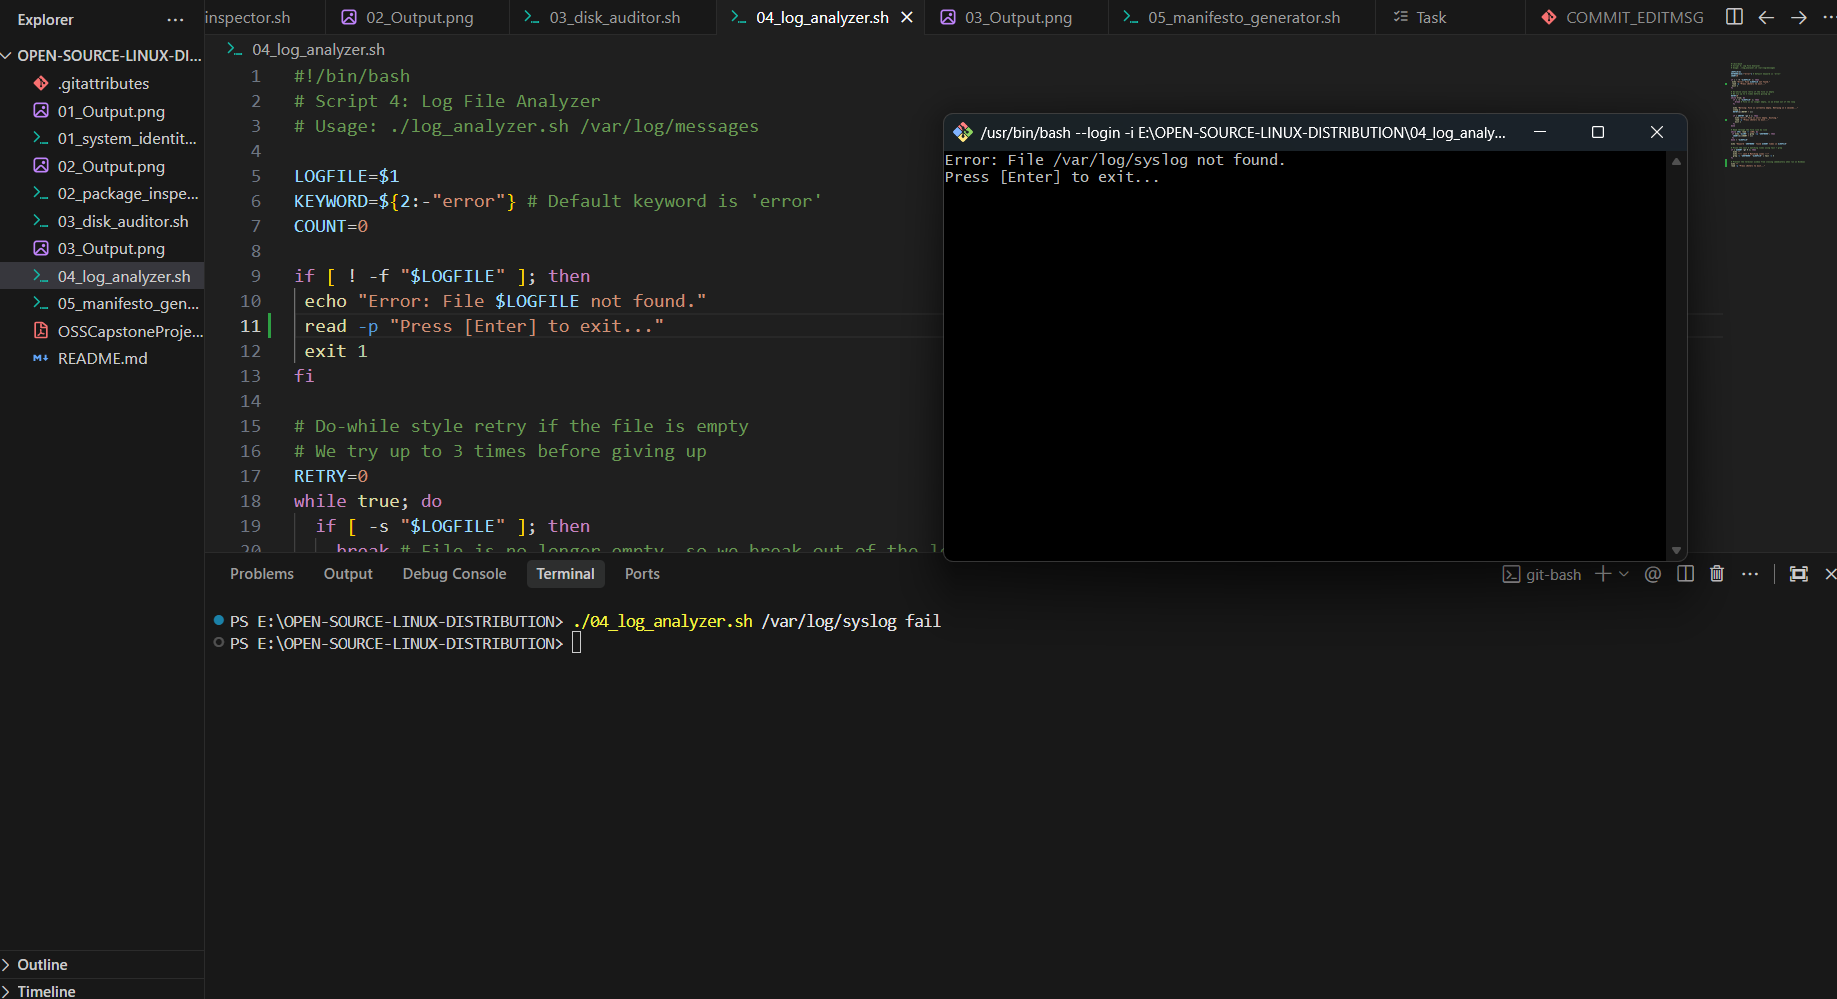
\includegraphics[width=\textwidth]{04_Output.png}
    \caption{Execution of Log File Analyzer utilizing loop evaluation.}
\end{figure}


\section{Script 5: Manifesto Generator}
This requests three unique inputs interactively. It logically concatenates those strings to completely write out a dynamic generated text file via redirection (\texttt{>>}). 

\begin{lstlisting}[language=bash, caption=05\_manifesto\_generator.sh]
#!/bin/bash
# Script 5: Open Source Manifesto Generator

echo "Answer three questions to generate your manifesto."
read -p "1. Name one open-source tool you use every day: " TOOL
read -p "2. In one word, what does 'freedom' mean to you? " FREEDOM
read -p "3. Name one thing you would build and share freely: " BUILD

DATE=$(date '+%d %B %Y')
OUTPUT="manifesto_$(whoami).txt"

echo "### My Open Source Manifesto ###" > "$OUTPUT"
echo "Date: $DATE" >> "$OUTPUT"
echo "I believe in open source because tools like $TOOL make my daily life easier." >> "$OUTPUT"
echo "To me, true freedom means $FREEDOM, which is exactly the core philosophy of open source." >> "$OUTPUT"
echo "If I had the chance to contribute, I would build $BUILD and share it!" >> "$OUTPUT"

echo "Manifesto saved to $OUTPUT"
cat "$OUTPUT"

echo ""
read -p "Press [Enter] to exit..."
\end{lstlisting}

\begin{figure}[H]
    \centering
    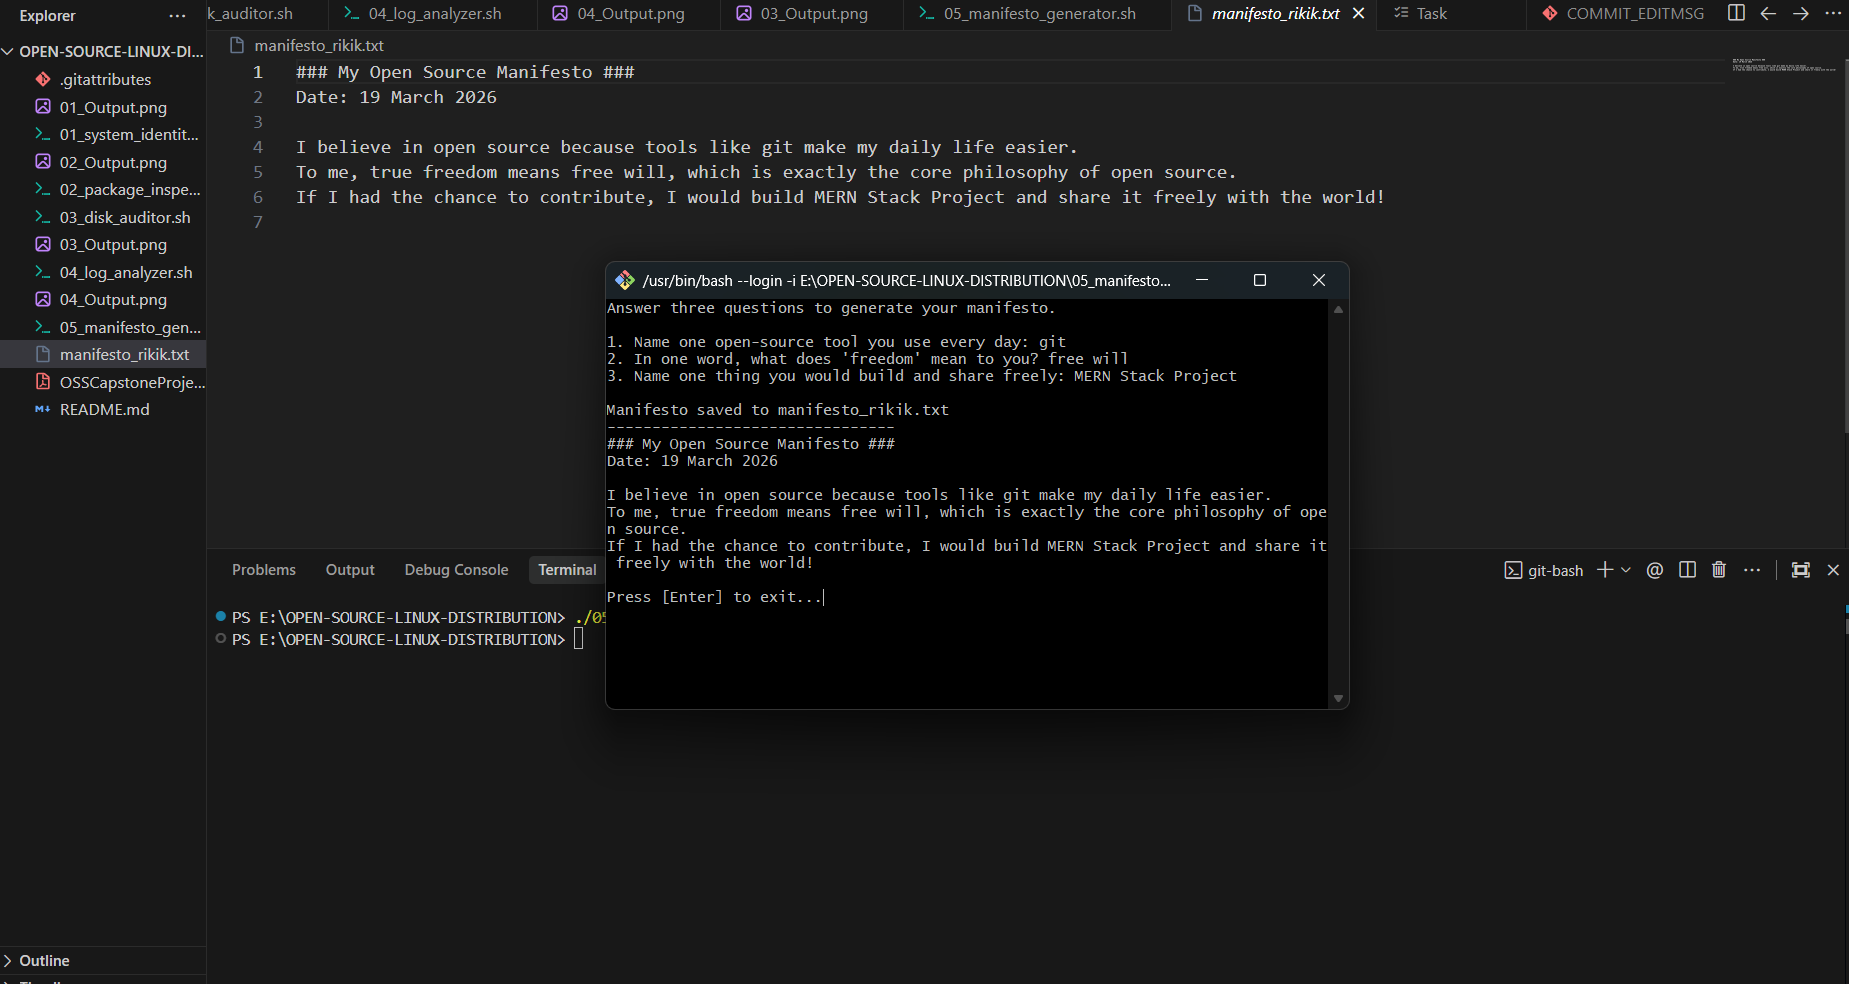
\includegraphics[width=\textwidth]{05_Output.png}
    \caption{Execution of Manifesto Generator handling text file I/O operations.}
\end{figure}


\chapter{Conclusion}
This assignment was highly illuminating. Before compiling this audit, my understanding of Linux and FOSS felt intimidating and entirely theoretical. Building out real functional automation scripts to audit system directories and dynamically parse software versions showed me the incredible connective power of the Linux CLI architecture. I finally learned that you don't always need to build extremely complex binary tools to engineer interesting behaviour; successfully chaining together lightweight operations like `awk`, `cut`, and `grep` creates resilient workflows.

Additionally, digging into the GPL ideology powering tools like Git made the history of modern programming significantly more obvious. Open source clearly isn't just charity or academic theory; it is the critical collaborative scaffolding that makes all large-scale internet tech possible. It is thrilling to realize that as my career grows, everything I construct will literally be running atop the silent, massive shoulders of these free community toolsets. 

\end{document}
